% 2001 年全国旧课程卷理科第 12 题：信息网络
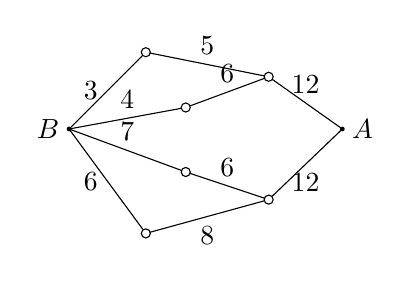
\begin{tikzpicture}[>=stealth, scale=0.78]
  \coordinate (B) at (0,0);
  \coordinate (U) at (1.25,1.25);
  \coordinate (V) at (3.25,0.85);
  \coordinate (M) at (1.9,0.35);
  \coordinate (N) at (1.9,-0.7);
  \coordinate (W) at (1.25,-1.7);
  \coordinate (Z) at (3.25,-1.15);
  \coordinate (A) at (4.45,0);

  \draw (B)--(U) node[midway, left] {3};
  \draw (U)--(V) node[midway, above] {5};
  \draw (B)--(M) node[midway, above] {4};
  \draw (M)--(V) node[midway, above] {6};
  \draw (B)--(N) node[midway, above] {7};
  \draw (N)--(Z) node[midway, above] {6};
  \draw (B)--(W) node[midway, left] {6};
  \draw (W)--(Z) node[midway, below] {8};
  \draw (V)--(A) node[midway, above] {12};
  \draw (Z)--(A) node[midway, below] {12};

  \foreach \point in {U,V,M,N,W,Z}
    \filldraw[fill=white] (\point) circle (2.1pt);
  \fill (B) circle (1.1pt) node[left] {$B$};
  \fill (A) circle (1.1pt) node[right] {$A$};
\end{tikzpicture}
